\documentclass[a4paper]{article}
\usepackage[version=4]{mhchem}
\usepackage{graphicx}
\usepackage[left = 3.18 cm, right = 3.18 cm, top = 2.54 cm, bottom = 2.54 cm]{geometry}
\usepackage{fancyhdr}
\usepackage{setspace}
\pagestyle{fancy}
\chead{ESE - ZHOU DAFU - U2407032}
\rhead{}
\onehalfspacing
\setlength{\parindent}{0pt}
\title{Research Plan of Final Year Project}
\date{}
\begin{document}
\maketitle
\begin{itemize}
    \item{Topic: Advanced oxidation methods for the treatment of landfill leachate wastewater}
    \item{Name: Zhou Dafu}
    \item{Number: U2407032}
    \item{Supervisor: Prof. Ong Say Leong}
    \item{Mentor: Wu Jiahua}
\end{itemize}

\section*{Abstract}

Landfill leachate is wastewater produced by landfills, characterized by its complex composition and resistance to degradation, which poses both direct and indirect threats to human health and the ecological environment. Due to their strong degradation capabilities, advanced oxidation processes (AOPs) can serve as an effective method for treating landfill leachate. This study aims to investigate the removal efficiency of various AOPs in landfill leachate treatment, while comparing and identifying the most efficient and cost-effective approach.

\section{Introduction}

Currently, landfills are the most widely used method for the disposal of solid waste. In China, over 80\% of the 160 million tonnes of municipal solid waste (MSW) generated in the same year was buried in 668 landfills{[}1{]}. Although landfills offer the advantages of operational simplicity and low costs, the waste undergoes physicochemical and biological transformations within the landfill, resulting in the generation of highly polluted secondary wastewater known as landfill leachate{[}2{]}. The composition of landfill leachate is highly complex, typically containing various organic pollutants, inorganic salts, toxic heavy metals, pathogens, and emerging contaminants (ECs). These components can pose direct or indirect threats to the ecological environment. For instance, the contamination of groundwater and drinking water by ECs such as pharmaceuticals and personal care products (PPCPs), and surfactants have been reported to pose a serious health risk to human beings and animals{[}3{]}. To evaluate the toxicity of landfill leachate, Baderna et al. (2019) established a cell model which confirmed that raw leachate causes irreversible damage to DNA repair enzymes and mechanisms. All these indicate that landfill leachate is a serious pollution issue threatening human health{[}4{]}. In this context, the effective treatment of landfill leachate has become an urgent research priority.

As traditional treatment methods, physical and biological technologies are widely applied, but each of these methods has notable shortcomings that limit their applicability. For instance, physical methods such as adsorption and coagulation cannot thoroughly eliminate the adverse impacts of leachate on the environment{[}5{]}; traditional biotechnology presents poor removal efficiency towards refractory compounds from aged landfill leachate{[}6{]}. In comparison to these traditional methods, the advanced oxidation processes (AOPs) demonstrate the advantage of stable system operation with the capability to process high organics loadings{[}4{]}. AOPs, through the action of hydroxyl and sulfate radicals, exhibit significantly higher degradation capacity than traditional methods, making them a promising solution for landfill leachate treatment.

This study will focus on comparing the degradation efficiency and costs of various AOPs. Furthermore, through mathematical methods such as statistical analysis and modeling, this research will analyze the correlation between changes in operational parameters and treatment outcomes as well as associated costs.

\section{Research Objectives}

\begin{enumerate}
    \item Analyze the removal or degradation efficiency of various contaminants in landfill leachate under different experimental conditions.  
    \item Ensure the stability and reproducibility of the optimal treatment conditions through single-factor and orthogonal experiments.  
    \item Explore the correlation between removal efficiency, cost, and operational parameters through statistical analysis.  
    \item Conduct a preliminary investigation into the foaming issue in landfill leachate.
\end{enumerate}

\section{Research Gaps}

\begin{enumerate}
    \item The specific impacts of varying operational parameters on the degradation outcomes of landfill leachate.
    \item Comprehensive cost-performance analysis of different advanced oxidation processes (AOPs).
\end{enumerate}

\section{Methodology}

The advanced oxidation process (AOP), primarily catalytic ozonation.

Ozone, as a powerful oxidizing agent, generates reactive species such as hydroxyl radicals, which can effectively attack and degrade large organic molecules in landfill leachate into smaller, more manageable compounds. The reaction mechanism is shown in Figure 1. However, due to the presence of side reactions and limitations in reaction rates, the degradation process often requires the use of catalysts. These catalysts enhance the reaction by increasing both the rate and selectivity, thereby improving the efficiency of ozone oxidation in treating leachate.
\begin{figure}[htb]
    \centering
    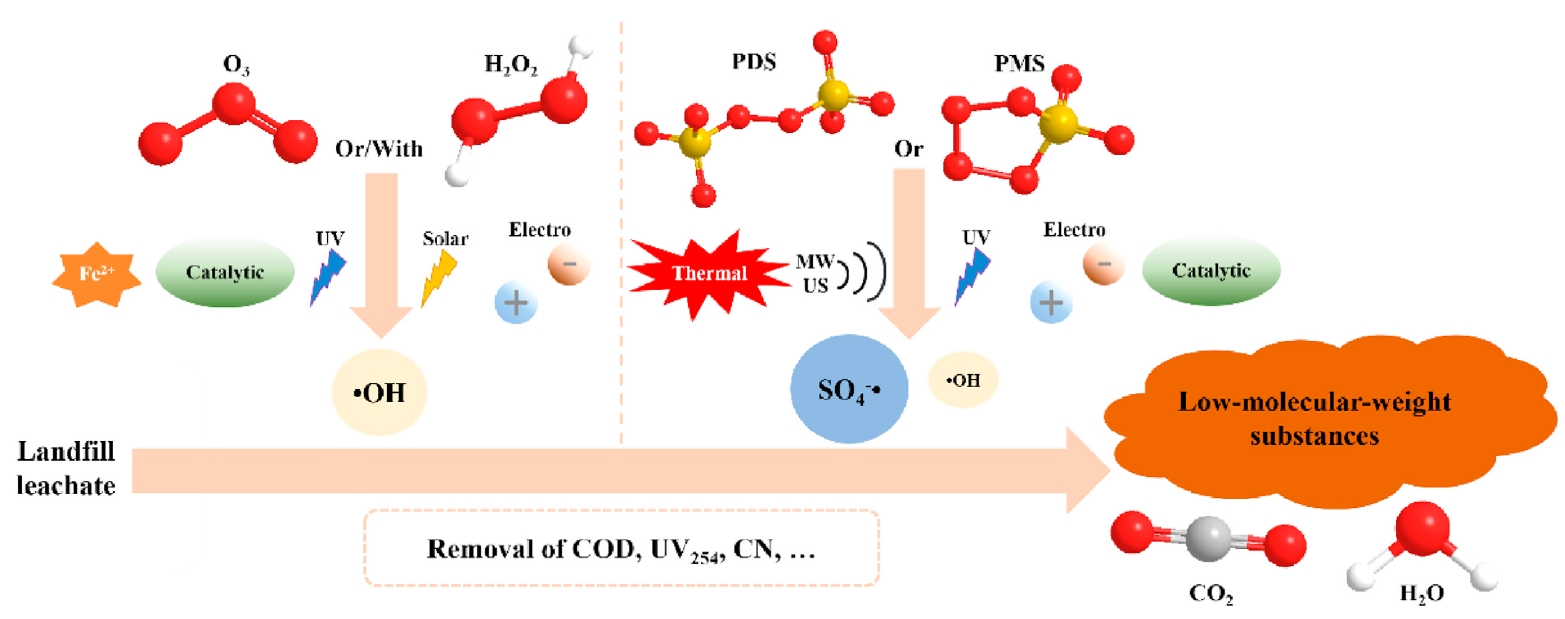
\includegraphics[width = .8\textwidth]{plan-1.png}
    \caption{Pathways of landfill leachate degradation by advanced oxidation processes[4]}
\end{figure}
\section{Research Content}
\subsection*{Part 1: Characterization of Pollutants in Landfill Leachate}

The initial phase involves a comprehensive characterization of the
landfill leachate to establish a baseline for treatment. Key parameters
such as pH, total organic carbon (TOC), chemical oxygen demand (COD),
biological oxygen demand (BOD5), color, total nitrogen (TN), ammonium
nitrogen ($\ce{NH4+}-\ce{N}$), heavy metal concentrations, and the presence of
emerging contaminants (ECs) like pharmaceuticals and personal care
products will be measured. This detailed analysis is crucial to
understand the complexity of the leachate and to identify the specific
contaminants that need to be targeted. National environmental standards
will serve as benchmarks to assess permissible pollutant levels and to
evaluate the effectiveness of subsequent treatment processes.
\subsection*{Part 2: Experimental Setup and Preparation}

Experimental reactors will be designed and assembled to facilitate
various advanced oxidation processes (AOPs), including catalytic
ozonation and Fenton oxidation. Necessary reagents and catalysts, such
as ozone generators, hydrogen peroxide ($\ce{H2O2}$), ferrous ions ($\ce{Fe2+}$), and
catalyst supports, will be prepared according to experimental
requirements. Safety protocols will be established for handling reactive
oxidants and operating equipment. Preliminary tests will be conducted to
ensure that the experimental apparatus functions correctly and that
measurement instruments are calibrated accurately.

\subsection*{Part 3: Single-Factor Experiments}

Single-factor experiments will be conducted to investigate the impact of individual operational parameters on pollutant removal efficiency. Variables such as initial pH, reaction time, oxidant dosage (e.g., ozone concentration, $\ce{H2O2}$ amount), catalyst loading, temperature, and mixing intensity will be systematically varied while other conditions remain constant. Landfill leachate samples will be treated under these varying conditions, and the effluent will be analyzed for changes in COD, TOC, color, TN, $\ce{NH4+}$-N, and specific contaminants identified in Part 1. The goal is to determine the optimal range for each parameter and to identify which factors have the most significant effect on treatment efficiency.

\subsection*{Part 4: Orthogonal Experiments}

Based on insights gained from the single-factor experiments, an orthogonal experimental design will be implemented to optimize the treatment conditions. Significant factors will be selected and arranged in an orthogonal array to evaluate multiple variables simultaneously with a reduced number of experiments. This statistical approach allows for the assessment of the main effects and interactions between factors. The effluent from each experimental run will be analyzed as before, and the data will be used to identify the combination of conditions that yields the highest pollutant removal efficiency. Statistical tools such as analysis of variance (ANOVA) will be employed to interpret the results and validate the optimal conditions.

\subsection*{Part 5: Continuous Testing and Stability Assessment}

To ensure the reliability and practical applicability of the optimized treatment conditions, continuous experiments will be conducted over an extended period. The stability and reproducibility of the AOPs under optimal conditions will be assessed by repeatedly treating fresh landfill leachate samples and monitoring pollutant removal efficiencies. Factors such as catalyst deactivation, potential formation of by-products, and operational robustness will be evaluated. This phase aims to confirm that the treatment process maintains high efficiency over time and is suitable for scaling up to industrial applications.

\subsection*{Part 6: Energy Consumption and Carbon Emission Analysis}

A critical aspect of the study is evaluating the energy demands of each AOP method and their associated carbon emissions. Energy consumption will be assessed by measuring the power required for generating ozone, mixing reagents, maintaining temperature, and other process-specific needs. This analysis will quantify the total energy usage for each method, offering a clear comparison between the processes. Additionally, carbon emissions will be calculated based on the energy consumption and the type of energy sources used. By examining both energy efficiency and carbon footprint, the study aims to identify the treatment method with the least environmental impact, which is crucial for sustainable landfill leachate management.

\subsection*{Part 7: Efficiency and Cost Analysis}

In parallel, the efficiency of each AOP method will be analyzed in relation to its operational costs. This will involve calculating the amount of reagent needed (such as ozone or hydrogen peroxide) to achieve optimal pollutant removal and comparing this with the corresponding treatment efficiency, such as COD reduction or contaminant degradation rates. Cost factors will include the price of chemicals, energy costs, and any additional expenses related to equipment or maintenance. By correlating efficiency with cost, the study will determine which AOP method offers the best balance between high pollutant removal rates and economic feasibility. This analysis is essential for scaling the technology to industrial applications, where both performance and cost must be optimized.

\newpage

\section{Annual Timetable}

\begin{table}[h!]
    \centering
    \begin{tabular}{|l|p{10cm}|}
    \hline
    \textbf{Time Period} & \textbf{Research Content} \\ \hline
    1 Oct to 14 Oct 2024 & Literature reading and consulting with mentor and supervisor to confirm the project theme \\ \hline
    15 Oct to 28 Oct 2024 & Initial pollutant analysis and experimental preparation, setting up reactors and reagents \\ \hline
    29 Oct to 11 Nov 2024 & Single-factor experiments: Assess impact of individual parameters on pollutant degradation \\ \hline
    12 Nov to 25 Nov 2024 & Orthogonal experiments: Explore optimal treatment conditions using multiple parameters \\ \hline
    26 Nov to 9 Dec 2024 & Continuous testing: Ensure stability and reproducibility of optimal conditions \\ \hline
    10 Dec to 23 Dec 2024 & Analysis of energy consumption and carbon emissions for different AOP methods \\ \hline
    24 Dec 2024 to 6 Jan 2025 & Efficiency and cost analysis: Evaluate cost-effectiveness of each method \\ \hline
    7 Jan to 17 Jan 2025 & Further analysis and prepare for mid-term presentation \\ \hline
    18 Jan to 16 Feb 2025 & Winter holiday \\ \hline
    17 Feb to 1 Mar 2025 & Continue experiments on energy consumption, carbon emissions, and optimization \\ \hline
    2 Mar to 15 Mar 2025 & Finalize results from continuous testing, refine efficiency and cost analysis \\ \hline
    16 Mar to 25 Mar 2025 & Prepare comprehensive data for final evaluation of AOPs \\ \hline
    26 Mar to 8 Apr 2025 & Essay writing \\ \hline
    9 Apr to 21 Apr 2025 & Final review of experimental results and essay refinement \\ \hline
    22 Apr to 15 May 2025 & FYP final assessment \\ \hline
    \end{tabular}
    \caption{Research Timetable}
\end{table}
    
\section{References}

{[}1{]} Z.Y. Feng, D. Na, L.J. Hong, X.C. Zhong, A new pyrolysis
technology and equipment for treatment of municipal household garbage
and hospital waste, Renewable Energy 28 (15) (2003) 2383--2393.

{[}2{]} Ghosh, P., Thakur, I. S., \& Kaushik, A. (2017). Bioassays for
toxicological risk assessment of landfill leachate: A review.
\emph{Ecotoxicology and Environmental Safety}, \emph{141}, 259--270.

{[}3{]} Pastore, C., Barca, E., Del Moro, G., Di Iaconi, C., Loos, M.,
Singer, H. P., \& Mascolo, G. (2018). Comparison of different types of
landfill leachate treatments by employment of nontarget screening to
identify residual refractory organics and principal component analysis.
\emph{Science of The Total Environment}, \emph{635}, 984--994.

{[}4{]} Li, S., Yang, Y., Zheng, H., Zheng, Y., Jing, T., Ma, J., Nan,
J., Leong, Y. K., \& Chang, J.-S. (2022). Advanced oxidation process
based on hydroxyl and sulfate radicals to degrade refractory organic
pollutants in landfill leachate. \emph{Chemosphere}, \emph{297}, 134214.

{[}5{]} Chen, G., Wu, G., Li, N., Lu, X., Zhao, J., He, M., Yan, B.,
Zhang, H., Duan, X., \& Wang, S. (2021). Landfill leachate treatment by
persulphate related advanced oxidation technologies. \emph{Journal of
Hazardous Materials}, \emph{418}, 126355.

{[}6{]} Tałałaj, I.A., Biedka, P., Bartkowska, I., 2019. Treatment of
landfill leachates with biological pretreatments and reverse osmosis.
Environ. Chem. Lett. 17 (3), 1177--1193.


\end{document}